\chapter{Empirical Comparison of Learning Algorithms}\label{ch:comparison}
In this chapter, we provide an empirical evaluation of the learning algorithms
described in Chapter~\ref{ch:structured_pystruct}.  We use the open source
implementations in \pystruct, and publish the evaluation code and datasets with
the package.

\section{Datasets and Models}
We consider several qualitatively different datasets that have been widely used in the literature.
The problems we consider are multi-class classification, sequence labeling, multi-label prediction,
and general graph labeling.

\subsection{Multi-Class Classification (MNIST)}
\begin{figure}
    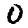
\includegraphics[width=.092\linewidth, frame]{evaluation/images/mnist_digit_0}
    
\includegraphics[width=.092\linewidth, frame]{evaluation/images/mnist_digit_1}
    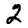
\includegraphics[width=.092\linewidth, frame]{evaluation/images/mnist_digit_2}
    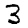
\includegraphics[width=.092\linewidth, frame]{evaluation/images/mnist_digit_3}
    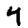
\includegraphics[width=.092\linewidth, frame]{evaluation/images/mnist_digit_4}
    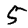
\includegraphics[width=.092\linewidth, frame]{evaluation/images/mnist_digit_5}
    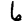
\includegraphics[width=.092\linewidth, frame]{evaluation/images/mnist_digit_6}
    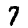
\includegraphics[width=.092\linewidth, frame]{evaluation/images/mnist_digit_7}
    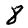
\includegraphics[width=.092\linewidth, frame]{evaluation/images/mnist_digit_8}
    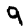
\includegraphics[width=.092\linewidth, frame]{evaluation/images/mnist_digit_9}
    \caption{%
        Visualization of samples from the ten classes in the MNIST dataset.\figlabel{mnist_illustration}
    }
\end{figure}
The simplest task we use is multi-class classification. In this task,
the inference problem is trivial, as it is assumed the target set is small enough
to be enumerated efficiently. While this problem could be solved more efficiently
with specialized algorithms, it nevertheless provides an initial insight into structured
prediction algorithms.
We choose the classical MNIST dataset of handwritten digits, consisting of
$60000$ training images and $10000$ test images of the digits zero to nine.
\Figref{mnist_illustration} shows some examples. Each image is a $28{\times}28$
grey-level image, resulting in a $784$-dimensional feature vector. We normalize
the features between $0$ and $1$.
%
\enlargethispage{15mm}
The model we use for multi-class classification is the Crammer-Singer
formulation. We do not include a bias, leading to $784 \cdot 10 = 7840$
parameters in the model.


\begin{figure}
    
\includegraphics[width=.068\linewidth, frame]{evaluation/images/justifications_00}
    
\includegraphics[width=.068\linewidth, frame]{evaluation/images/justifications_01}
    
\includegraphics[width=.068\linewidth, frame]{evaluation/images/justifications_02}
    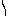
\includegraphics[width=.068\linewidth, frame]{evaluation/images/justifications_03}
    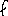
\includegraphics[width=.068\linewidth, frame]{evaluation/images/justifications_04}
    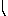
\includegraphics[width=.068\linewidth, frame]{evaluation/images/justifications_05}
    
\includegraphics[width=.068\linewidth, frame]{evaluation/images/justifications_06}
    
\includegraphics[width=.068\linewidth, frame]{evaluation/images/justifications_07}
    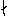
\includegraphics[width=.068\linewidth, frame]{evaluation/images/justifications_08}
    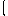
\includegraphics[width=.068\linewidth, frame]{evaluation/images/justifications_09}
    
\includegraphics[width=.068\linewidth, frame]{evaluation/images/justifications_10}
    
\includegraphics[width=.068\linewidth, frame]{evaluation/images/justifications_11}
    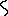
\includegraphics[width=.068\linewidth, frame]{evaluation/images/justifications_12}\\[3mm]
    
\includegraphics[width=.068\linewidth, frame]{evaluation/images/skiing_00}
    
\includegraphics[width=.068\linewidth, frame]{evaluation/images/skiing_01}
    
\includegraphics[width=.068\linewidth, frame]{evaluation/images/skiing_02}
    
\includegraphics[width=.068\linewidth, frame]{evaluation/images/skiing_03}
    
\includegraphics[width=.068\linewidth, frame]{evaluation/images/skiing_04}\\[3mm]
    
\includegraphics[width=.068\linewidth, frame]{evaluation/images/unexpected_00}
    
\includegraphics[width=.068\linewidth, frame]{evaluation/images/unexpected_01}
    
\includegraphics[width=.068\linewidth, frame]{evaluation/images/unexpected_02}
    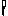
\includegraphics[width=.068\linewidth, frame]{evaluation/images/unexpected_03}
    
\includegraphics[width=.068\linewidth, frame]{evaluation/images/unexpected_04}
    
\includegraphics[width=.068\linewidth, frame]{evaluation/images/unexpected_05}
    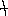
\includegraphics[width=.068\linewidth, frame]{evaluation/images/unexpected_06}
    
\includegraphics[width=.068\linewidth, frame]{evaluation/images/unexpected_07}
    
\includegraphics[width=.068\linewidth, frame]{evaluation/images/unexpected_08}\\
    \caption{%
        Visualization of some words from the OCR dataset. The first letters were removed by \citet{taskar2003max} as 
        they were capitals.
        The words are: (j)ustifications, (s)kiing and (u)nexpected. The letters in parentheses are not part of the dataset.
        \figlabel{ocr_illustration}
    }
\end{figure}
\subsection{Sequence Labeling (OCR)}
A classical application of structured prediction is sequence labeling.
We choose the ``OCR'' dataset introduced in the seminal work of \citet{taskar2003max}.
Each input consists of the segmented handwritten letters of a word in lower
case. The task is to classify all letters in a word, that is, assign each
segmented input letter to one of the classes ``a'' to ``z''. As the first letter
of each word was capitalized, these were removed by \citet{taskar2003max},
leading to somewhat odd-looking labels. The words are between three and fourteen
letters long, and each letter is represented as a binary image of size $16
\time 8$, with a total of $6877$ words.
The dataset is divided into ten folds. We consider two setups: learning
on one fold, and testing on the remaining nine folds, following \citet{taskar2003max},
and learning on nine folds and testing on the remaining fold, following \citet{lacoste2012block}.
We refer to the learning on one fold as \textsc{OCR-small}, and learning on nine folds as OCR-big.
We use a simple chain model with a single constant pairwise feature.
This means that the unary potential has $16 \cdot 8 \cdot 26 = 768$ parameters, one for each input
feature and output class. The pairwise potential consists of a matrix of
transition potentials with $26 \cdot 26=676$ entries.
It is well-known that efficient exact inference in chains is possible using
message passing algorithms. 


\subsection{Multi-Label Classification}
Multi-label classification is a generalization of multi-class classification,
in which each example can be associated with more than one class. In other
words, the algorithm must decide for each sample and for each class whether the
sample belongs to that class or not.
Multi-label classification was first formulated as a structured prediction problem
by \citet{finley2008training}, who used to investigate the influence of
approximate inference on the $n$-slack cutting plane algorithm. In their formulation
each class is represented as a binary node in a factor graph---the states representing
presence or absence of the class. A different factor of pairwise potentials is introduced
between each pair of classes.
We also consider a different model, where pairwise potentials are only
introduced between specific nodes. We build a tree over the binary variables by
computing the Chow-Liu Tree~\citep{chow1968approximating} of the targets. While
this results in a less expressive model, a tree-shaped model allows for exact
inference via message passing.
We use two of the datasets used in \citet{finley2008training}, the \textsc{scene}
and \textsc{yeast} datasets. We choose these two as these are real-world datasets for
which the pairwise approach outlined above actually improves upon the
baseline~\citep{finley2008training}.
The \textsc{scene} dataset has six labels, 294 input features, 1211 training samples and
1196 test samples. This leads to $204 \cdot 6 = 1224$ parameters for the unary potentials,
$3 \cdot 5 \cdot 4 = 60$ parameters for the full pairwise potentials (four for each edge), and
$5 \cdot 4 = 20$ parameters for the pairwise potentials of the tree-shaped model.
Using four parameters for each edge is a slight over-parametrization that
simplifies writing out the model.
The \textsc{yeast} dataset has 14 labels, 103 features, 1500 training samples and 971
test samples. The resulting numbers of parameters are $14 \cdot 103=1442$ parameters
for the unary potentials, $7 \cdot 13 \cdot 4=364$ parameters for the full pairwise
potential, and $13 \cdot 4=52$ parameters for the tree-shaped model.

\begin{figure}
    \begin{tabu} to \linewidth{@{}XXXXXXX@{}}
    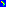
\includegraphics[width=\linewidth]{evaluation/images/snake_input_0001}&%
    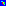
\includegraphics[width=\linewidth]{evaluation/images/snake_input_0002}&%
    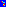
\includegraphics[width=\linewidth]{evaluation/images/snake_input_0003}&%
    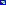
\includegraphics[width=\linewidth]{evaluation/images/snake_input_0004}&%
    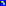
\includegraphics[width=\linewidth]{evaluation/images/snake_input_0005}&%
    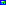
\includegraphics[width=\linewidth]{evaluation/images/snake_input_0006}&%
    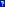
\includegraphics[width=\linewidth]{evaluation/images/snake_input_0007}\\
    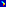
\includegraphics[width=\linewidth]{evaluation/images/snake_label_0001}&%
    
\includegraphics[width=\linewidth]{evaluation/images/snake_label_0002}&%
    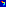
\includegraphics[width=\linewidth]{evaluation/images/snake_label_0003}&%
    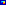
\includegraphics[width=\linewidth]{evaluation/images/snake_label_0004}&%
    
\includegraphics[width=\linewidth]{evaluation/images/snake_label_0005}&%
    
\includegraphics[width=\linewidth]{evaluation/images/snake_label_0006}&%
    \includegraphics[width=\linewidth]{evaluation/images/snake_label_0007}
    \end{tabu}
\caption{%
    Visualization of the \textsc{snakes} dataset. The top row shows input patterns, the bottom row the corresponding
    labels. The colors in the image showing the labels correspond to dark blue for background, and encoding
    the length of the snake from head (red) to tail (blue).
\figlabel{snakes_illustration}}
\end{figure}

\subsection{2D Grid CRF (Snakes)}
The \textsc{snakes} dataset is a synthetic dataset where samples are labeled 2D grids.
It was introduced by \citet{nowozin2011decision} to demonstrate the importance
of learning conditional pairwise potentials. The dataset consists of ``snakes''
of length ten traversing the 2D grid. Each grid cell that was visited is marked
as the snake heading out towards the top, bottom, left, or right, while
unvisited cells are marked as background.  The goal is to predict a labeling of
the snake from ``head'' to ``tail'', that is, assigning numbers from zero to
nine to the cells that are occupied by the snake.  \Figref{snakes_illustration}
illustrates the principle.
Local evidence for the target label is weak except
around head and tail, making this a challenging task, requiring strong pairwise
potentials. The dataset is noise-free in the sense that given the above
description, a human could easily produce the desired labeling without making
any mistake. The dataset is also interesting as the model proposed by
\citet{nowozin2011decision} produced notoriously hard-to-optimize energy
functions.

Originally, the input is encoded into five RGB colors
(``up'', ``down'', ``left'', ``right'', ``background'').  To encode the input
more suitably for our linear methods, we convert this representation to a
one-hot encoding of the five states.

We use a grid CRF model for this task. Unary potentials for each node are given by the
input of the 8-neighborhood of the node---using a 4-neighborhood would most
likely yield better results, but we do not want to encode too much
task-knowledge into our model.
Using the one-hot encoding of the input, this leads to $9 \cdot 5 = 45$ unary features.
With 11 output classes, the unary potential has $11 \cdot 9 \cdot 5=495$ parameters.
Features for the pairwise potentials are constructed by concatenating the features
of the two neighboring nodes, taking the direction of the edge into account.
The pairwise feature therefore has dimensionality $45 \cdot 4$, with the first
$45$ entries corresponding to the feature of the ``top'' node, the second $45$
entries to the features ``bottom'' node, followed by the ``left'' and
``right'' nodes. As each edge is either horizontal \emph{or} vertical, only two
of these parts will be non-zero for any given edge.  With $45 \cdot 4$ edge
features, the pairwise potentials have $45 \cdot 4 \cdot 11^2 =21780$ parameters.


\subsection{Superpixel CRFs for Semantic Segmentation}
Our main attention is devoted to the use of conditional random fields for
semantic segmentation.  We use the \textsc{Pascal VOC} and MSRC datasets.
The \textsc{Pascal VOC} has 964 training images, each divided into
around 100 superpixels. There are 20 object categories, and an additional background class. The % TODO check! refer to other part
MSRC-21 dataset has 276 training images, also segmented in around 100 superpixels
each. There are 21 classes in the MSRC-21 dataset.
Each superpixel is represented as an output variable, with the ground truth
obtained by majority vote over the pixels belonging to the superpixel. We
removed all superpixels in which the majority of pixels is labeled ``void'', leading to some samples
having much fewer than 100 variables.
Pairwise potentials are introduced for each pair of neighboring superpixels.
We use the unary and pairwise potentials described in \Secref{semantic_segmentation}:
21 unary features for the \textsc{Pascal VOC} dataset and 63 unary features for the MSRC-21 dataset.
We use the same three pairwise features for both datasets: a constant feature, a color
feature and a feature encoding relative vertical position.
Overall, this results in $21 \cdot  21 + 3 \cdot 21 \cdot 21 = 1764$ parameters
for the potentials on \textsc{Pascal VOC} and $63 \cdot  21 + 3 \cdot 21 \cdot 21 =
2646$ parameters for the potentials on the MSRC-21 dataset.

%For Pascal VOC we use the probabilities provided by
%\citet{krahenbuhl2012efficient}, which combine low-level Texton-Boost
%potentials with bounding-box object detectors.  We average probabilities inside
%each superpixel, yielding 21 input features for both datasets.  We also used
%the
%same pairwise features for the two datasets: a constant feature, a color
%contrast feature, and a feature encoding relative vertical position between
%superpixels.  Overall, the models for both datasets had $21 \cdot 21 + 21^2
%\cdot 4$ features.  It is possible to assume symmetric potentials for this
%dataset, leading to less pairwise features. We found both parametrizations
%yielded similar results.

\begin{table}
    \begin{tabu} to \linewidth{@{}X[1,l]YX[1,c]X[1,c]YY@{}}
    %\multicolumn{2}{@{}c@{}}{\includegraphics[width=\linewidth]{evaluation/legend.pdf}}\\
    \toprule
    Dataset             & {samples} & variables & graph & {dim $\theta$} & {labels}\\
    \cmidrule{1-6}
    MNIST               & 60000   & 1     & none  & 7840  & 10\\
    \textsc{OCR-small}  & 704     & 3--14 & chain & 1444  & 26\\
    \textsc{OCR-large}  & 6173    & 3--14 & chain & 1444  & 26\\
    \textsc{scene-tree} & 1211    & 6     & tree  & 1244  & 2\\
    \textsc{scene-full} & 1211    & 6     & loopy & 1284  & 2\\
    \textsc{yeast-tree} & 1500    & 14    & tree  & 1494  & 2\\
    \textsc{yeast-full} & 1500    & 14    & loopy & 1806  & 2\\
    \textsc{snakes}     & 200     &84--168& loopy & 22275 & 11\\
    MSRC-21             & 276     & 7--113& loopy &  1764 & 21\\
    \textsc{Pascal VOC} & 964     & 8--112& loopy &  2646 & 21\\
    \bottomrule
    \end{tabu}
    \caption{Summary of datasets used in the evaluation. \tablabel{datasets}}
\end{table}

\section{Experiments}
We compare the following algorithms on the above models (see \Secref{learning_algorithms} for details):
\begin{itemize}
    \item Stochastic Subgradient Descent (SSGD) using the Pegasos schedule for step-sizes
    %\item Stochastic Subgradient Descent using the Pegasos schedule: AVERAGING
    \item The $1$-slack cutting plane algorithm without inference caching
    \item The $1$-slack cutting plane algorithm with caching the last 50
        inference results for each sample (see Chapter~\ref{ch:exact_learning}
        for details)
    \item The $n$-slack cutting plane algorithm, where the QP is solved after each sample
    \item The $n$-slack cutting plane algorithm, where the QP is solved every 100 samples
    \item The SZLJSP algorithm with weighted averaging
\end{itemize}

All algorithms take a $C$ parameter, which we adjusted on a fully trained model
on a validation set (experiments not reported here) and held constant for all
models.  We found, however, that the algorithms and models are quite robust to
the choice of $C$ within one or two orders of magnitude.
As stopping criterion, we used a duality gap of $0.1$ when possible, and a
pre-defined number of iterations for the subgradient algorithms. It is worth
noting that the quadratic programming based algorithms have additional
hyper-parameters that we do not discuss here in detail, such as the threshold
for removing a constraint as inactive, how often inactive constraints are
removed, and parameters of the underlying QP solver. On the other hand, the
SZLJSP algorithm, has no hyper-parameters except for the stopping criterion.

Our ultimate evaluation criterion is how fast the learning algorithms converge,
and how robust they are to approximate inference.  To quantify our goals, we
track primal suboptimality and training set error during learning.
%, as well as final error on the test set. FIXME?
We report primal suboptimality as a function of runtime, and as a function of passes
over the training set.  Both are informative to practitioners, as they give
important insight into the working of the algorithm.  The actual runtime is
arguably the most relevant factor, but also highly influenced by
implementation details and properties of the dataset. We are particularly
interested in cases where inference is highly non-trivial, making it the
dominating factor with respect to runtime.
We define one pass over the dataset as calling prediction once for each sample.
This way, we can get a clear picture of how learning times scale with complexity of the
inference task. For the subgradient and SZLJSP algorithms, learning time is linear
in the number of passes over the dataset, while caching and solving of a QP makes
the learning time depend on the number of iterations in hard-to-predict ways.
All algorithms were run on a single core i7 processor.

\subsection{Experiments using Exact Inference}
In this section, we present results on multi-class classification, sequence
labeling and multi-label prediction. In these tasks, exact inference is
possible, and we can compute the exact objective of the various algorithms
easily. We use the dynamic programming algorithm implemented in \textsc{OpenGM}
for experiments for the tree and chain models.
For the full pairwise multi-label model, we use branch-and-bound together with
the AD$^3$ algorithm. %FIXME AD3 solver description?
We found that using the linear programming relaxation on the \textsc{scene} dataset is
often tight, and there was no need to resort to approximate inference. Inference
on the \textsc{yeast} dataset was more complex, and on the verge of being non-practical.
We use this dataset as an example for very costly inference.

\begin{figure}
    \begin{tabu} to \linewidth{@{}XX@{}}
    \multicolumn{2}{@{}c@{}}{\includegraphics[width=\linewidth]{evaluation/legend.pdf}}\\[-3mm]
    \includegraphics[width=\linewidth]{evaluation/images/mnist}&%
    \includegraphics[width=\linewidth]{evaluation/images/mnist_loss}
    \end{tabu}
\caption{%
   Convergence of the primal suboptimality and training set loss on MNIST. 
\figlabel{mnist_curves}}
\end{figure}

We start our experiments with the MNIST dataset.
The convergence of the primal suboptimality and training set loss in terms of
passes over the training set is shown in \Figref{mnist_curves}. While inference
is trivial, this is by far the largest dataset, making the $n$-slack algorithms
not feasible. We see that the stochastic algorithms are much faster than the
cutting plane algorithm, in particular initially, even in terms of iterations,
with the SZLJSP clearly leading the way.
Interestingly, the $1$-slack algorithm catches up near the desired
suboptimality.  Looking at the training set loss in \Figref{mnist_curves}
suggests that the high precision we demanded was not necessary, and we could
have terminated the stochastic algorithms much earlier.



\begin{figure}
    \begin{tabu} to \linewidth{@{}XX@{}}
    \multicolumn{2}{@{}c@{}}{\includegraphics[width=\linewidth]{evaluation/legend.pdf}}\\[-3mm]
    \includegraphics[width=\linewidth]{evaluation/images/letters_small_log}&%
    \includegraphics[width=\linewidth]{evaluation/images/letters_small_log_time}
    \end{tabu}
\caption{%
   Convergence of the primal suboptimality on OCR-small. 
\figlabel{ocr_small_results}}
\end{figure}

We now consider datasets with non-trivial inference.
The results for \textsc{OCR-small} are shown in \Figref{ocr_small_results}.
Considering the plot against passes over the dataset on the left, several
trends can be observed: the $n$-slack cutting plane algorithms converge
fastest, with the version that recomputes the QP at every step leading the
race. The algorithms are closely followed by the caching $1$-slack cutting
plane algorithm.  They are followed by the significantly slower SZLJSP
algorithm, and finally the non-caching $1$-slack cutting plane algorithm and
subgradient descent.  These results are intuitive, as they reflect ``how much
work'' each algorithm does for each loss-augmented prediction step. More work
towards the objective leads to faster convergence.  This ``more work'' is
quantified on the right hand side of \Figref{ocr_small_results}, where the suboptimality is plotted against time.
Clearly the $n$-slack algorithms do ``too much'' work, leading to very slow
convergence.  Also, caching does not speed up learning learning on this
dataset.
 
We want to highlight an interesting phenomenon here: The cutting-plane
algorithms stop immediately when reaching the desired suboptimality of $0.1$.
The SZLJSP algorithm, on the other hand, keeps on learning much longer---even
though the primal of the $1$-slack algorithms is always above the primal of the
SZLJSP\@. This is caused by a looser bound given by the dual. Remember that the
stopping criterion for both cutting-plane and SZLJSP are given by the duality
gap. It seems that while the primal objective converges much faster in the
SZLJSP algorithm than in the non-caching $1$-slack algorithm, the dual does
not. This means that in this practical experiment, the non-caching $1$-slack
algorithm was \emph{faster} in guaranteeing the desired suboptimality, and
therefore in terminating.  \Figref{ocr_small_dual} illustrates this point by
plotting primal and dual objectives for the $1$-slack cutting plane and the
SZLJSP algorithms. Taking a closer look, we find that the same behavior
occurred for MNIST, which is also shown in \Figref{ocr_small_dual}.

%The trends seen in the figures are similar to what we saw for MNIST above.
%Again, even though inference is non-trivial, the non-caching $1$-slack
%algorithm is slower than the caching one. Again, the plots against passes over the training set
%do not reflect the runtime complexity of the $n$-slack approach.

\begin{figure}
    \begin{tabu} to \linewidth{@{}XX@{}}
    \multicolumn{2}{@{}c@{}}{\includegraphics[width=\linewidth]{evaluation/legend.pdf}}\\[-3mm]
    \includegraphics[width=\linewidth]{evaluation/images/mnist_duality_gap}&%
    \includegraphics[width=\linewidth]{evaluation/images/letters_small_duality_gap}
    \end{tabu}
\caption{%
    Primal objective and dual objective (dashed lines) for SZLJSP and $1$-slack cutting plane on MNIST (left) and \textsc{OCR-small} (right).
\figlabel{ocr_small_dual}}
\end{figure}


\begin{figure}
    \begin{tabu} to \linewidth{@{}XX@{}}
    \multicolumn{2}{@{}c@{}}{\includegraphics[width=\linewidth]{evaluation/legend.pdf}}\\[-3mm]
    \includegraphics[width=\linewidth]{evaluation/images/letters_big_log}&%
    \includegraphics[width=\linewidth]{evaluation/images/letters_big_log_time}
    \end{tabu}
\caption{%
   Convergence of the primal suboptimality on OCR-large. 
\figlabel{ocr_large_results}}
\end{figure}

The results for the OCR-large dataset are shown in \Figref{ocr_large_results}. It was not feasible to run the $n$-slack
algorithm when solving the QP at every step here.
The trends are the same as for the smaller dataset: $n$-slack and caching $1$-slack cutting plane are very fast
in terms of passes through the dataset, but $n$-slack cutting plane is impractical slow
with respect to runtime. The SZLJSP algorithm converges fast initially, but the $1$-slack cutting plane
is faster at high precision and faster in certifying the desired duality gap.
\begin{figure}
    \begin{tabu} to \linewidth{@{}XX@{}}
    \multicolumn{2}{@{}c@{}}{\includegraphics[width=\linewidth]{evaluation/legend.pdf}}\\[-3mm]
    \includegraphics[width=\linewidth]{evaluation/images/scene_tree_log}&%
    \includegraphics[width=\linewidth]{evaluation/images/scene_tree_log_time}\\
    \includegraphics[width=\linewidth]{evaluation/images/scene_full_log}&%
    \includegraphics[width=\linewidth]{evaluation/images/scene_full_log_time}\\
    \includegraphics[width=\linewidth]{evaluation/images/yeast_tree_log}&%
    \includegraphics[width=\linewidth]{evaluation/images/yeast_tree_log_time}\\
    \includegraphics[width=\linewidth]{evaluation/images/yeast_full}&%
    \includegraphics[width=\linewidth]{evaluation/images/yeast_full_time}
    \end{tabu}
\caption{%
   Convergence of the primal suboptimality on the multi-label datasets. From top to
   bottom: the \textsc{scene} dataset using a tree model, the \textsc{scene} dataset using a full
   model, the \textsc{yeast} dataset using a tree model, and the \textsc{yeast} dataset using a
   full model.
\figlabel{multi-label-results}}
\end{figure}

Next, we consider the multi-label task.  The results for the \textsc{yeast} and \textsc{scene}
datasets are shown in \Figref{multi-label-results}. The caching $1$-slack
algorithm is much faster than the non-caching one on both datasets and both
graph structures.
While the two variants of the $n$-slack algorithm are equally fast with respect
to passes over the training data, solving the QP every 100 steps is among the
fastest algorithms, while solving the QP at every step is among the slowest.
We applied this method only to the smaller \textsc{scene} dataset, as applying it on the
\textsc{yeast} dataset was not practical.

The caching $1$-slack algorithm is the fastest algorithm to achieve the desired
primal suboptimality for tree-structured graphs, while it is out-performed by
the $n$-slack cutting plane algorithm for the full graphs. This is intuitive,
as the additional work the $n$-slack algorithm does becomes more valuable, the
longer the inference takes. 


%, inference is much more complex than in the previous tasks.

\subsection{Experiments using Approximate Inference}
For the remaining tasks, the \textsc{snakes} dataset and image segmentation, exact
inference is intractable for learning.
%
We use two different approximate inference algorithms, fusion moves, a fast
local search procedure, and the linear programming relaxation provided by AD$^3$
not using branch-and-bound, in contrast to the multi-label setup above.

Evaluation of algorithms where exact inference is not possible is much harder,
as it is usually not possible to evaluate the exact objective. When using AD$^3$,
we can still consider the relaxed task, which will be solved exactly in the
majority of cases (AD$^3$ can fail to find the primal solution to the LP
relaxation).
When using fusion moves, there is no obvious interpretation of the approximate
primal objective, other than that it provides a lower bound of the actual
objective. Nevertheless, we find it informative to analyze the behavior of this
lower bound. In contrast to the previous section, we show primal and dual objective
values instead of the primal suboptimality when using approximate inference.
The dual values do provide lower bounds
to the exact objective, and are therefore somewhat more informative here, see
Chapter~\ref{ch:exact_learning} for a discussion.

For both inference algorithms, we also evaluate the predictive performance on
the training set.  We explicitly do not consider the relaxed problem
here---instead we round possible fractional results. While the training error
does not directly reflect the objective, it provides a measure of how effective
the ``prediction machine'' given by the learned model together with the
inference algorithm is.

\Figref{snakes_results} shows the results on the \textsc{snakes} dataset.
The top row shows the objective when learning with fusion moves, the next row
the training set loss.  First, we observe that using fusion moves, even the
approximate objective does not reach the desired optimality gap for the
$1$-slack and SZLJSP algorithms. This is caused by the algorithms not finding
any further constraints. The $n$-slack algorithm fares a bit better and
achieves a higher dual value. Looking at the training set loss, it is clear that the stochastic
algorithms have an advantage, possibly caused by not stopping too early.
Still, all algorithms ultimately fail to solve the task.

The situation is very different when using the linear programming relaxation.
Looking at the four plots at the bottom of \Figref{snakes_results}, we see that all
algorithms are able to solve the task perfectly. Evaluating on the test-set, all algorithms
achieve an accuracy of around 99.5\%, confirming the models actually learned the task.
Surprisingly, SSGD was very successful on this dataset, even faster then the non-caching $n$-slack
algorithm. Caching provides nearly an order of magnitude speed-up on the dataset.
%
Using branch-and-bound to obtain exact results was not feasible on this dataset.

\begin{figure}
    \begin{tabu} to \linewidth{@{}XX@{}}
    \multicolumn{2}{@{}c@{}}{\includegraphics[width=\linewidth]{evaluation/legend.pdf}}\\[-3mm]
    \includegraphics[width=\linewidth]{evaluation/images/snakes_qpbo}&%
    \includegraphics[width=\linewidth]{evaluation/images/snakes_qpbo_time}\\
    \includegraphics[width=\linewidth]{evaluation/images/snakes_qpbo_loss}&%
    \includegraphics[width=\linewidth]{evaluation/images/snakes_qpbo_time_loss}\\
    \includegraphics[width=\linewidth]{evaluation/images/snakes_ad3}&%
    \includegraphics[width=\linewidth]{evaluation/images/snakes_ad3_time}\\
    \includegraphics[width=\linewidth]{evaluation/images/snakes_ad3_loss}&%
    \includegraphics[width=\linewidth]{evaluation/images/snakes_ad3_time_loss}
    \end{tabu}
\caption{%
    Results on the \textsc{snakes} dataset. The top four plots show results using fusion
    move inference, the bottom four plots using AD$^3$. Dashed lines indicate the dual objective.
\figlabel{snakes_results}}
\end{figure}

The last set of experiments is on the segmentation dataset MSRC-21 and \textsc{Pascal
VOC}.  Because of the large number of labels and samples, it is only feasible
to use the fusion move inference algorithm. The results are shown in
\Figref{msrc_pascal_curves}, with the top four plots showing results on
MSRC-21, and the bottom four plots showing results on \textsc{Pascal VOC}.
First, we notice that all algorithms achieve low (approximate) duality gaps, and none
of the algorithms terminates prematurely. Also, all algorithms achieve a
similar dual objectives and similar training errors after convergence.
In both datasets, the $1$-slack algorithm is somewhat slow in minimizing the
training set error, and the $n$-slack and stochastic algorithms are much
faster. Solving the QP only every 100 steps in the $n$-slack algorithm significantly slows
down learning on both datasets. This is in contrast to the \textsc{yeast} datasets, where the converse was true,
even though \textsc{yeast} has a similar number of training examples to \textsc{Pascal VOC}.

Given the outcome described above, we suspect that learning was not affected by approximate
inference too much. We leave a more detailed analysis for Chapter~\ref{ch:exact_learning}.\pagebreak\\

\begin{figure}
    \begin{tabu} to \linewidth{@{}XX@{}}
    \multicolumn{2}{@{}c@{}}{\includegraphics[width=\linewidth]{evaluation/legend.pdf}}\\[-3mm]
    \includegraphics[width=\linewidth]{evaluation/images/msrc}&%
    \includegraphics[width=\linewidth]{evaluation/images/msrc_time}\\
    \includegraphics[width=\linewidth]{evaluation/images/msrc_loss}&%
    \includegraphics[width=\linewidth]{evaluation/images/msrc_time_loss}\\
    \includegraphics[width=\linewidth]{evaluation/images/pascal}&%
    \includegraphics[width=\linewidth]{evaluation/images/pascal_time}\\
    \includegraphics[width=\linewidth]{evaluation/images/pascal_loss}&%
    \includegraphics[width=\linewidth]{evaluation/images/pascal_time_loss}
    \end{tabu}
\caption{%
    Objective and traning set loss on the segmentation task. The top four plots
    show results for the MSRC-21 dataset, the bottom four plots for the \textsc{Pascal
    VOC} dataset.
\figlabel{msrc_pascal_curves}}
\end{figure}

\section{Summary}
From the experiments above, it is clear there is currently \emph{no single best algorithm}.
However, there are some clear trends:
\begin{itemize}
    \item SZLJSP always converges faster than SSGD, with each iteration having
        the same time complexity.  This indicates that SZLJSP should be
        preferred over SSGD, apart from settings with strong memory
        constraints.
    \item In nearly all experiments, caching significantly improved performance
        of the 1-slack cutting plane algorithm.
    \item Initially SZLJSP and even SSGD converge faster than the 1-slack
        cutting plane algorithm, while the 1-slack cutting plane algorithm was
        faster in achieving high precision solutions and guaranteeing low
        duality gap.
    \item The $n$-slack cutting plane algorithm was often fastest to converge in
        terms of passes over the training set, but slow in terms of
        runtime. For problems with very slow inference, the $n$-slack algorithm
        might be a better choice than the others---if the interval between re-solving
        the QP is chosen appropriately.
\end{itemize}
There are however some caveats to our analysis, in particular with respect to
the cutting plane solvers. The performance of the cutting plane algorithms
depends not only on the performance of the QP solver used (in our case
quadratic cone programming), but also on heuristics for pruning variables from
the QP, caching constraints (for the $1$-slack algorithm) and deciding how
often to solve the QP (for the $n$-slack algorithm). Better heuristics could
have a beneficial effect on these algorithms. On the other hand, it is
remarkable how competitive the SZLJSP algorithm is, without the need for any
such implementation tricks. This makes the SZLJSP algorithm very attractive for
the practitioner who does not want to spend much time tuning the
implementation.

We do not present results for SSGD with averaging~\citep{lacoste2012simpler} here, but
found it to produce results similar to plain SSGD in tentative experiments. In
particular, it never outperformed SZLJSP.

With respect to approximate learning, we found that the inference algorithm has
a stronger impact on the performance than the learning algorithm.
While the SSGD and SZLJSP algorithms have somewhat lower training error on the \textsc{snakes} dataset than
the cutting-plane algorithm when using fusion-move inference, they, too, fail at solving the task.
Using the linear programming relaxation, on the other hand, all algorithms are able to solve the
task nearly perfectly.
For the segmentation datasets, it is harder to judge the outcome, though there
seems to be little difference between the learning algorithms in terms of the
final result.  In the next chapter, we will demonstrate how we can learn
exactly, even with the complex models used for semantic segmentation.
